% Options for packages loaded elsewhere
\PassOptionsToPackage{unicode}{hyperref}
\PassOptionsToPackage{hyphens}{url}
%
\documentclass[
]{article}
\usepackage{amsmath,amssymb}
\usepackage{iftex}
\ifPDFTeX
  \usepackage[T1]{fontenc}
  \usepackage[utf8]{inputenc}
  \usepackage{textcomp} % provide euro and other symbols
\else % if luatex or xetex
  \usepackage{unicode-math} % this also loads fontspec
  \defaultfontfeatures{Scale=MatchLowercase}
  \defaultfontfeatures[\rmfamily]{Ligatures=TeX,Scale=1}
\fi
\usepackage{lmodern}
\ifPDFTeX\else
  % xetex/luatex font selection
\fi
% Use upquote if available, for straight quotes in verbatim environments
\IfFileExists{upquote.sty}{\usepackage{upquote}}{}
\IfFileExists{microtype.sty}{% use microtype if available
  \usepackage[]{microtype}
  \UseMicrotypeSet[protrusion]{basicmath} % disable protrusion for tt fonts
}{}
\makeatletter
\@ifundefined{KOMAClassName}{% if non-KOMA class
  \IfFileExists{parskip.sty}{%
    \usepackage{parskip}
  }{% else
    \setlength{\parindent}{0pt}
    \setlength{\parskip}{6pt plus 2pt minus 1pt}}
}{% if KOMA class
  \KOMAoptions{parskip=half}}
\makeatother
\usepackage{xcolor}
\usepackage[margin=1in]{geometry}
\usepackage{color}
\usepackage{fancyvrb}
\newcommand{\VerbBar}{|}
\newcommand{\VERB}{\Verb[commandchars=\\\{\}]}
\DefineVerbatimEnvironment{Highlighting}{Verbatim}{commandchars=\\\{\}}
% Add ',fontsize=\small' for more characters per line
\usepackage{framed}
\definecolor{shadecolor}{RGB}{248,248,248}
\newenvironment{Shaded}{\begin{snugshade}}{\end{snugshade}}
\newcommand{\AlertTok}[1]{\textcolor[rgb]{0.94,0.16,0.16}{#1}}
\newcommand{\AnnotationTok}[1]{\textcolor[rgb]{0.56,0.35,0.01}{\textbf{\textit{#1}}}}
\newcommand{\AttributeTok}[1]{\textcolor[rgb]{0.13,0.29,0.53}{#1}}
\newcommand{\BaseNTok}[1]{\textcolor[rgb]{0.00,0.00,0.81}{#1}}
\newcommand{\BuiltInTok}[1]{#1}
\newcommand{\CharTok}[1]{\textcolor[rgb]{0.31,0.60,0.02}{#1}}
\newcommand{\CommentTok}[1]{\textcolor[rgb]{0.56,0.35,0.01}{\textit{#1}}}
\newcommand{\CommentVarTok}[1]{\textcolor[rgb]{0.56,0.35,0.01}{\textbf{\textit{#1}}}}
\newcommand{\ConstantTok}[1]{\textcolor[rgb]{0.56,0.35,0.01}{#1}}
\newcommand{\ControlFlowTok}[1]{\textcolor[rgb]{0.13,0.29,0.53}{\textbf{#1}}}
\newcommand{\DataTypeTok}[1]{\textcolor[rgb]{0.13,0.29,0.53}{#1}}
\newcommand{\DecValTok}[1]{\textcolor[rgb]{0.00,0.00,0.81}{#1}}
\newcommand{\DocumentationTok}[1]{\textcolor[rgb]{0.56,0.35,0.01}{\textbf{\textit{#1}}}}
\newcommand{\ErrorTok}[1]{\textcolor[rgb]{0.64,0.00,0.00}{\textbf{#1}}}
\newcommand{\ExtensionTok}[1]{#1}
\newcommand{\FloatTok}[1]{\textcolor[rgb]{0.00,0.00,0.81}{#1}}
\newcommand{\FunctionTok}[1]{\textcolor[rgb]{0.13,0.29,0.53}{\textbf{#1}}}
\newcommand{\ImportTok}[1]{#1}
\newcommand{\InformationTok}[1]{\textcolor[rgb]{0.56,0.35,0.01}{\textbf{\textit{#1}}}}
\newcommand{\KeywordTok}[1]{\textcolor[rgb]{0.13,0.29,0.53}{\textbf{#1}}}
\newcommand{\NormalTok}[1]{#1}
\newcommand{\OperatorTok}[1]{\textcolor[rgb]{0.81,0.36,0.00}{\textbf{#1}}}
\newcommand{\OtherTok}[1]{\textcolor[rgb]{0.56,0.35,0.01}{#1}}
\newcommand{\PreprocessorTok}[1]{\textcolor[rgb]{0.56,0.35,0.01}{\textit{#1}}}
\newcommand{\RegionMarkerTok}[1]{#1}
\newcommand{\SpecialCharTok}[1]{\textcolor[rgb]{0.81,0.36,0.00}{\textbf{#1}}}
\newcommand{\SpecialStringTok}[1]{\textcolor[rgb]{0.31,0.60,0.02}{#1}}
\newcommand{\StringTok}[1]{\textcolor[rgb]{0.31,0.60,0.02}{#1}}
\newcommand{\VariableTok}[1]{\textcolor[rgb]{0.00,0.00,0.00}{#1}}
\newcommand{\VerbatimStringTok}[1]{\textcolor[rgb]{0.31,0.60,0.02}{#1}}
\newcommand{\WarningTok}[1]{\textcolor[rgb]{0.56,0.35,0.01}{\textbf{\textit{#1}}}}
\usepackage{graphicx}
\makeatletter
\def\maxwidth{\ifdim\Gin@nat@width>\linewidth\linewidth\else\Gin@nat@width\fi}
\def\maxheight{\ifdim\Gin@nat@height>\textheight\textheight\else\Gin@nat@height\fi}
\makeatother
% Scale images if necessary, so that they will not overflow the page
% margins by default, and it is still possible to overwrite the defaults
% using explicit options in \includegraphics[width, height, ...]{}
\setkeys{Gin}{width=\maxwidth,height=\maxheight,keepaspectratio}
% Set default figure placement to htbp
\makeatletter
\def\fps@figure{htbp}
\makeatother
\setlength{\emergencystretch}{3em} % prevent overfull lines
\providecommand{\tightlist}{%
  \setlength{\itemsep}{0pt}\setlength{\parskip}{0pt}}
\setcounter{secnumdepth}{-\maxdimen} % remove section numbering
\ifLuaTeX
  \usepackage{selnolig}  % disable illegal ligatures
\fi
\IfFileExists{bookmark.sty}{\usepackage{bookmark}}{\usepackage{hyperref}}
\IfFileExists{xurl.sty}{\usepackage{xurl}}{} % add URL line breaks if available
\urlstyle{same}
\hypersetup{
  pdftitle={Laboratorio 5},
  pdfauthor={Keneth Ruiz},
  hidelinks,
  pdfcreator={LaTeX via pandoc}}

\title{Laboratorio 5}
\author{Keneth Ruiz}
\date{2023-09-26}

\begin{document}
\maketitle

\begin{Shaded}
\begin{Highlighting}[]
\FunctionTok{library}\NormalTok{(lubridate)}
\end{Highlighting}
\end{Shaded}

\begin{verbatim}
## 
## Attaching package: 'lubridate'
\end{verbatim}

\begin{verbatim}
## The following objects are masked from 'package:base':
## 
##     date, intersect, setdiff, union
\end{verbatim}

\begin{Shaded}
\begin{Highlighting}[]
\FunctionTok{library}\NormalTok{(readxl)}
\FunctionTok{library}\NormalTok{(dplyr)}
\end{Highlighting}
\end{Shaded}

\begin{verbatim}
## 
## Attaching package: 'dplyr'
\end{verbatim}

\begin{verbatim}
## The following objects are masked from 'package:stats':
## 
##     filter, lag
\end{verbatim}

\begin{verbatim}
## The following objects are masked from 'package:base':
## 
##     intersect, setdiff, setequal, union
\end{verbatim}

\begin{Shaded}
\begin{Highlighting}[]
\FunctionTok{library}\NormalTok{(nycflights13)}
\FunctionTok{library}\NormalTok{(ggplot2)}
\FunctionTok{library}\NormalTok{(forecast)}
\end{Highlighting}
\end{Shaded}

\begin{verbatim}
## Registered S3 method overwritten by 'quantmod':
##   method            from
##   as.zoo.data.frame zoo
\end{verbatim}

\hypertarget{parte-1}{%
\subsection{Parte 1}\label{parte-1}}

\begin{Shaded}
\begin{Highlighting}[]
\NormalTok{eclipse\_inicial }\OtherTok{\textless{}{-}} \FunctionTok{dmy\_hms}\NormalTok{(}\StringTok{\textquotesingle{}21 aug 2017 18:26:40\textquotesingle{}}\NormalTok{)}
\NormalTok{synodic\_month }\OtherTok{\textless{}{-}} \FunctionTok{days}\NormalTok{(}\DecValTok{29}\NormalTok{)}\SpecialCharTok{+}\FunctionTok{hours}\NormalTok{(}\DecValTok{12}\NormalTok{)}\SpecialCharTok{+}\FunctionTok{minutes}\NormalTok{(}\DecValTok{44}\NormalTok{)}\SpecialCharTok{+}\FunctionTok{seconds}\NormalTok{(}\DecValTok{3}\NormalTok{)}
\NormalTok{saros }\OtherTok{\textless{}{-}}\NormalTok{ synodic\_month }\SpecialCharTok{*} \DecValTok{223}

\NormalTok{prox\_eclipse }\OtherTok{\textless{}{-}}\NormalTok{ eclipse\_inicial }\SpecialCharTok{\%m+\%}\NormalTok{ saros}
\NormalTok{prox\_eclipse}
\end{Highlighting}
\end{Shaded}

\begin{verbatim}
## [1] "2035-09-02 02:09:49 UTC"
\end{verbatim}

\hypertarget{parte-2}{%
\subsubsection{PARTE 2}\label{parte-2}}

\begin{Shaded}
\begin{Highlighting}[]
\CommentTok{\#Pura limpieza de datos con las fechas}
\NormalTok{data }\OtherTok{\textless{}{-}} \FunctionTok{read\_excel}\NormalTok{(}\StringTok{"data.xlsx"}\NormalTok{)}
\NormalTok{data }\OtherTok{\textless{}{-}}\NormalTok{ data[data}\SpecialCharTok{$}\NormalTok{Cod }\SpecialCharTok{!=} \DecValTok{0}\NormalTok{,]}
\NormalTok{convertir\_fecha }\OtherTok{\textless{}{-}} \ControlFlowTok{function}\NormalTok{(fecha) \{}
  \FunctionTok{tryCatch}\NormalTok{(}
\NormalTok{    \{}
      \FunctionTok{return}\NormalTok{(}\FunctionTok{as.Date}\NormalTok{(fecha, }\AttributeTok{format =} \StringTok{"\%d{-}\%m{-}\%y"}\NormalTok{))}
\NormalTok{    \},}
    \AttributeTok{error =} \ControlFlowTok{function}\NormalTok{(e) \{}
      \FunctionTok{return}\NormalTok{(}\ConstantTok{NA}\NormalTok{)  }
\NormalTok{    \}}
\NormalTok{  )}
\NormalTok{\}}
\NormalTok{data}\SpecialCharTok{$}\StringTok{\textasciigrave{}}\AttributeTok{Fecha Creación}\StringTok{\textasciigrave{}} \OtherTok{\textless{}{-}} \FunctionTok{convertir\_fecha}\NormalTok{(data}\SpecialCharTok{$}\StringTok{\textasciigrave{}}\AttributeTok{Fecha Creación}\StringTok{\textasciigrave{}}\NormalTok{)}
\NormalTok{data}\SpecialCharTok{$}\StringTok{\textasciigrave{}}\AttributeTok{Fecha Final}\StringTok{\textasciigrave{}} \OtherTok{\textless{}{-}} \FunctionTok{convertir\_fecha}\NormalTok{(data}\SpecialCharTok{$}\StringTok{\textasciigrave{}}\AttributeTok{Fecha Final}\StringTok{\textasciigrave{}}\NormalTok{)}
\NormalTok{data }\OtherTok{\textless{}{-}}\NormalTok{ data[}\SpecialCharTok{!}\FunctionTok{is.na}\NormalTok{(data}\SpecialCharTok{$}\StringTok{\textasciigrave{}}\AttributeTok{Fecha Creación}\StringTok{\textasciigrave{}}\NormalTok{), ]}
\end{Highlighting}
\end{Shaded}

\begin{Shaded}
\begin{Highlighting}[]
\CommentTok{\#Pregunta 2.1}
\NormalTok{meses\_con\_mas\_llamadas }\OtherTok{\textless{}{-}}\NormalTok{ data }\SpecialCharTok{\%\textgreater{}\%}
  \FunctionTok{group\_by}\NormalTok{(Cod, }\AttributeTok{Mes =} \FunctionTok{month}\NormalTok{(}\StringTok{\textasciigrave{}}\AttributeTok{Fecha Creación}\StringTok{\textasciigrave{}}\NormalTok{, }\AttributeTok{label =} \ConstantTok{TRUE}\NormalTok{)) }\SpecialCharTok{\%\textgreater{}\%}
  \FunctionTok{summarize}\NormalTok{(}\AttributeTok{Cantidad =} \FunctionTok{sum}\NormalTok{(Call), }\AttributeTok{.groups =} \StringTok{"drop"}\NormalTok{) }\SpecialCharTok{\%\textgreater{}\%}
  \FunctionTok{arrange}\NormalTok{(Cod, }\FunctionTok{desc}\NormalTok{(Cantidad))}
\FunctionTok{print}\NormalTok{(meses\_con\_mas\_llamadas)}
\end{Highlighting}
\end{Shaded}

\begin{verbatim}
## # A tibble: 72 x 3
##    Cod                          Mes   Cantidad
##    <chr>                        <ord>    <dbl>
##  1 Actualización de Información may        314
##  2 Actualización de Información mar        306
##  3 Actualización de Información dic        300
##  4 Actualización de Información ago        298
##  5 Actualización de Información oct        290
##  6 Actualización de Información jul        289
##  7 Actualización de Información nov        289
##  8 Actualización de Información ene        284
##  9 Actualización de Información sep        272
## 10 Actualización de Información jun        265
## # i 62 more rows
\end{verbatim}

\begin{Shaded}
\begin{Highlighting}[]
\CommentTok{\# Pregunta 2.2: Qué día de la semana es el más ocupado}
\NormalTok{dia\_ocupado }\OtherTok{\textless{}{-}}\NormalTok{ data }\SpecialCharTok{\%\textgreater{}\%}
  \FunctionTok{mutate}\NormalTok{(}\AttributeTok{dia\_semana =} \FunctionTok{weekdays}\NormalTok{(}\StringTok{\textasciigrave{}}\AttributeTok{Fecha Creación}\StringTok{\textasciigrave{}}\NormalTok{)) }\SpecialCharTok{\%\textgreater{}\%}
  \FunctionTok{group\_by}\NormalTok{(dia\_semana) }\SpecialCharTok{\%\textgreater{}\%}
  \FunctionTok{summarize}\NormalTok{(}\AttributeTok{Cantidad =} \FunctionTok{n}\NormalTok{(), }\AttributeTok{.groups =} \StringTok{\textquotesingle{}drop\textquotesingle{}}\NormalTok{) }\SpecialCharTok{\%\textgreater{}\%}
  \FunctionTok{arrange}\NormalTok{(}\FunctionTok{desc}\NormalTok{(Cantidad))}

\CommentTok{\# Imprimir los resultados en la terminal}
\FunctionTok{print}\NormalTok{(dia\_ocupado)}
\end{Highlighting}
\end{Shaded}

\begin{verbatim}
## # A tibble: 7 x 2
##   dia_semana Cantidad
##   <chr>         <int>
## 1 lunes         21715
## 2 viernes       21671
## 3 martes        21618
## 4 jueves        21582
## 5 sábado        21074
## 6 miércoles     20974
## 7 domingo       20870
\end{verbatim}

\begin{Shaded}
\begin{Highlighting}[]
\CommentTok{\# Pregunta 2.3: Qué mes es el más ocupado}
\NormalTok{meses\_ocupados }\OtherTok{\textless{}{-}}\NormalTok{ data }\SpecialCharTok{\%\textgreater{}\%}
  \FunctionTok{group\_by}\NormalTok{(}\AttributeTok{Mes =} \FunctionTok{month}\NormalTok{(}\StringTok{\textasciigrave{}}\AttributeTok{Fecha Creación}\StringTok{\textasciigrave{}}\NormalTok{, }\AttributeTok{label =} \ConstantTok{TRUE}\NormalTok{)) }\SpecialCharTok{\%\textgreater{}\%}
  \FunctionTok{summarize}\NormalTok{(}\AttributeTok{Cantidad =} \FunctionTok{n}\NormalTok{()) }\SpecialCharTok{\%\textgreater{}\%}
  \FunctionTok{arrange}\NormalTok{(}\FunctionTok{desc}\NormalTok{(Cantidad))}

\CommentTok{\# Imprimir los resultados en la terminal}
\FunctionTok{print}\NormalTok{(meses\_ocupados)}
\end{Highlighting}
\end{Shaded}

\begin{verbatim}
## # A tibble: 12 x 2
##    Mes   Cantidad
##    <ord>    <int>
##  1 oct      12953
##  2 ene      12951
##  3 mar      12946
##  4 may      12885
##  5 jul      12832
##  6 dic      12825
##  7 ago      12804
##  8 sep      12315
##  9 nov      12217
## 10 abr      12210
## 11 jun      11983
## 12 feb      10583
\end{verbatim}

\begin{Shaded}
\begin{Highlighting}[]
\CommentTok{\#pregunta 2.4 Crear un gráfico de líneas para visualizar tendencias estacionales}
\FunctionTok{ggplot}\NormalTok{(data, }\FunctionTok{aes}\NormalTok{(}\AttributeTok{x =} \StringTok{\textasciigrave{}}\AttributeTok{Fecha Creación}\StringTok{\textasciigrave{}}\NormalTok{, }\AttributeTok{y =}\NormalTok{ Call)) }\SpecialCharTok{+}
  \FunctionTok{geom\_line}\NormalTok{() }\SpecialCharTok{+}
  \FunctionTok{labs}\NormalTok{(}
    \AttributeTok{title =} \StringTok{"Tendencia Estacional en la Cantidad de Llamadas"}\NormalTok{,}
    \AttributeTok{x =} \StringTok{"Fecha"}\NormalTok{,}
    \AttributeTok{y =} \StringTok{"Cantidad de Llamadas"}
\NormalTok{  )}
\end{Highlighting}
\end{Shaded}

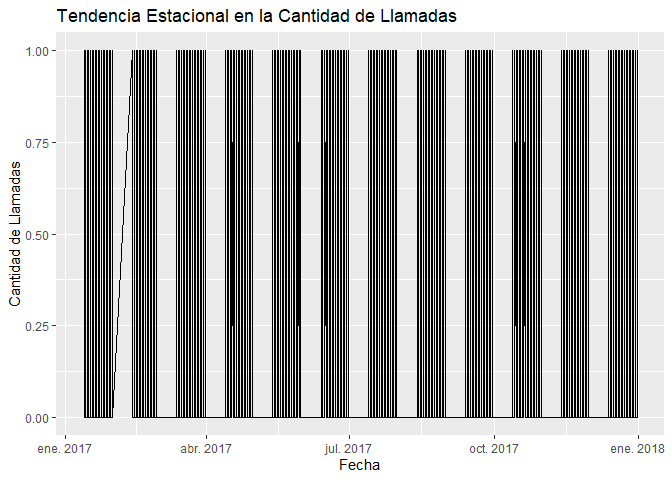
\includegraphics{Lab5_files/figure-latex/unnamed-chunk-6-1.pdf}

\begin{Shaded}
\begin{Highlighting}[]
\CommentTok{\# Realizar un análisis de descomposición de series temporales}
\FunctionTok{library}\NormalTok{(forecast)}

\NormalTok{ts\_data }\OtherTok{\textless{}{-}} \FunctionTok{ts}\NormalTok{(data}\SpecialCharTok{$}\NormalTok{Call, }\AttributeTok{frequency =} \DecValTok{12}\NormalTok{)  }\CommentTok{\# Suponiendo datos mensuales}
\NormalTok{decomp }\OtherTok{\textless{}{-}} \FunctionTok{decompose}\NormalTok{(ts\_data)}

\CommentTok{\# Visualizar los componentes de la descomposición}
\FunctionTok{plot}\NormalTok{(decomp)}
\end{Highlighting}
\end{Shaded}

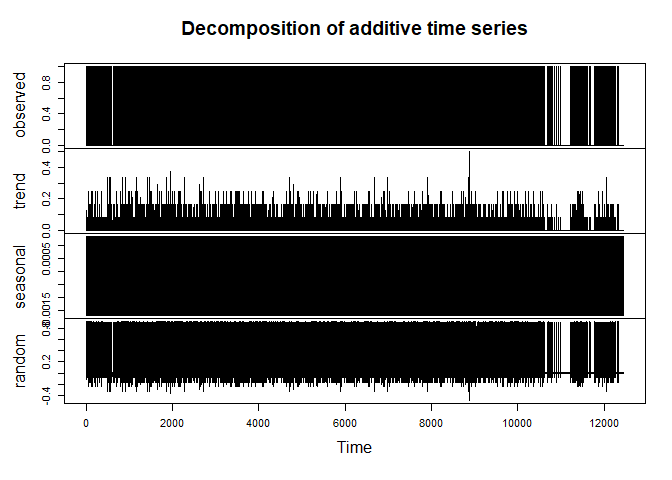
\includegraphics{Lab5_files/figure-latex/unnamed-chunk-6-2.pdf}

\begin{Shaded}
\begin{Highlighting}[]
\CommentTok{\# Pregunta 2.5: Cuántos minutos dura la llamada promedio}
\NormalTok{data}\SpecialCharTok{$}\NormalTok{duracion }\OtherTok{\textless{}{-}} \FunctionTok{as.numeric}\NormalTok{(}\FunctionTok{difftime}\NormalTok{(data}\SpecialCharTok{$}\StringTok{\textasciigrave{}}\AttributeTok{Hora Final}\StringTok{\textasciigrave{}}\NormalTok{, data}\SpecialCharTok{$}\StringTok{\textasciigrave{}}\AttributeTok{Hora Creación}\StringTok{\textasciigrave{}}\NormalTok{, }\AttributeTok{units =} \StringTok{"mins"}\NormalTok{))}
\NormalTok{duracion\_promedio }\OtherTok{\textless{}{-}} \FunctionTok{mean}\NormalTok{(data}\SpecialCharTok{$}\NormalTok{duracion[data}\SpecialCharTok{$}\NormalTok{Call }\SpecialCharTok{==} \DecValTok{1}\NormalTok{], }\AttributeTok{na.rm =} \ConstantTok{TRUE}\NormalTok{)  }
\FunctionTok{cat}\NormalTok{(}\StringTok{"La llamada promedio dura:"}\NormalTok{, duracion\_promedio, }\StringTok{"minutos}\SpecialCharTok{\textbackslash{}n}\StringTok{"}\NormalTok{)}
\end{Highlighting}
\end{Shaded}

\begin{verbatim}
## La llamada promedio dura: 14.61654 minutos
\end{verbatim}

\begin{Shaded}
\begin{Highlighting}[]
\CommentTok{\# Redondear la duración de llamadas al minuto más cercano}
\NormalTok{data}\SpecialCharTok{$}\NormalTok{duracion\_minutos }\OtherTok{\textless{}{-}} \FunctionTok{round}\NormalTok{(data}\SpecialCharTok{$}\NormalTok{duracion)}

\CommentTok{\# Crear una tabla de frecuencias}
\NormalTok{tabla\_frecuencias }\OtherTok{\textless{}{-}} \FunctionTok{table}\NormalTok{(data}\SpecialCharTok{$}\NormalTok{duracion\_minutos)}

\CommentTok{\# Convertir la tabla en un data frame}
\NormalTok{df\_tabla\_frecuencias }\OtherTok{\textless{}{-}} \FunctionTok{as.data.frame}\NormalTok{(tabla\_frecuencias)}

\CommentTok{\# Renombrar las columnas}
\FunctionTok{colnames}\NormalTok{(df\_tabla\_frecuencias) }\OtherTok{\textless{}{-}} \FunctionTok{c}\NormalTok{(}\StringTok{"Tiempo de Llamada en Minutos"}\NormalTok{, }\StringTok{"Cantidad de Llamadas"}\NormalTok{)}

\CommentTok{\# Imprimir la tabla de frecuencias}
\FunctionTok{print}\NormalTok{(df\_tabla\_frecuencias)}
\end{Highlighting}
\end{Shaded}

\begin{verbatim}
##    Tiempo de Llamada en Minutos Cantidad de Llamadas
## 1                             0                 5439
## 2                             1                 4909
## 3                             2                 4865
## 4                             3                 4832
## 5                             4                 4828
## 6                             5                 4800
## 7                             6                 4945
## 8                             7                 4734
## 9                             8                 4894
## 10                            9                 4786
## 11                           10                 4708
## 12                           11                 4772
## 13                           12                 4763
## 14                           13                 4876
## 15                           14                 4848
## 16                           15                 4927
## 17                           16                 4775
## 18                           17                 4941
## 19                           18                 4714
## 20                           19                 4736
## 21                           20                 4872
## 22                           21                 4612
## 23                           22                 4718
## 24                           23                 4835
## 25                           24                 4837
## 26                           25                 4634
## 27                           26                 4832
## 28                           27                 4853
## 29                           28                 4679
## 30                           29                 4761
## 31                           30                 4779
\end{verbatim}

\hypertarget{parte-3}{%
\subsubsection{PARTE 3}\label{parte-3}}

\begin{Shaded}
\begin{Highlighting}[]
\CommentTok{\#Pregunta 3.1}
\NormalTok{obtener\_signo\_zodiacal\_iso }\OtherTok{\textless{}{-}} \ControlFlowTok{function}\NormalTok{(fecha\_nacimiento) \{}
\NormalTok{  fecha }\OtherTok{\textless{}{-}} \FunctionTok{ymd}\NormalTok{(fecha\_nacimiento)}
\NormalTok{  mes\_dia }\OtherTok{\textless{}{-}} \FunctionTok{month}\NormalTok{(fecha) }\SpecialCharTok{*} \DecValTok{100} \SpecialCharTok{+} \FunctionTok{day}\NormalTok{(fecha)}
  
  \ControlFlowTok{if}\NormalTok{ ((mes\_dia }\SpecialCharTok{\textgreater{}=} \DecValTok{321} \SpecialCharTok{\&\&}\NormalTok{ mes\_dia }\SpecialCharTok{\textless{}=} \DecValTok{419}\NormalTok{)) \{}
    \FunctionTok{return}\NormalTok{(}\StringTok{"Aries"}\NormalTok{)}
\NormalTok{  \} }\ControlFlowTok{else} \ControlFlowTok{if}\NormalTok{ (mes\_dia }\SpecialCharTok{\textgreater{}=} \DecValTok{420} \SpecialCharTok{\&\&}\NormalTok{ mes\_dia }\SpecialCharTok{\textless{}=} \DecValTok{520}\NormalTok{) \{}
    \FunctionTok{return}\NormalTok{(}\StringTok{"Tauro"}\NormalTok{)}
\NormalTok{  \} }\ControlFlowTok{else} \ControlFlowTok{if}\NormalTok{ (mes\_dia }\SpecialCharTok{\textgreater{}=} \DecValTok{521} \SpecialCharTok{\&\&}\NormalTok{ mes\_dia }\SpecialCharTok{\textless{}=} \DecValTok{620}\NormalTok{) \{}
    \FunctionTok{return}\NormalTok{(}\StringTok{"Géminis"}\NormalTok{)}
\NormalTok{  \} }\ControlFlowTok{else} \ControlFlowTok{if}\NormalTok{ (mes\_dia }\SpecialCharTok{\textgreater{}=} \DecValTok{621} \SpecialCharTok{\&\&}\NormalTok{ mes\_dia }\SpecialCharTok{\textless{}=} \DecValTok{722}\NormalTok{) \{}
    \FunctionTok{return}\NormalTok{(}\StringTok{"Cáncer"}\NormalTok{)}
\NormalTok{  \} }\ControlFlowTok{else} \ControlFlowTok{if}\NormalTok{ (mes\_dia }\SpecialCharTok{\textgreater{}=} \DecValTok{723} \SpecialCharTok{\&\&}\NormalTok{ mes\_dia }\SpecialCharTok{\textless{}=} \DecValTok{822}\NormalTok{) \{}
    \FunctionTok{return}\NormalTok{(}\StringTok{"Leo"}\NormalTok{)}
\NormalTok{  \} }\ControlFlowTok{else} \ControlFlowTok{if}\NormalTok{ (mes\_dia }\SpecialCharTok{\textgreater{}=} \DecValTok{823} \SpecialCharTok{\&\&}\NormalTok{ mes\_dia }\SpecialCharTok{\textless{}=} \DecValTok{922}\NormalTok{) \{}
    \FunctionTok{return}\NormalTok{(}\StringTok{"Virgo"}\NormalTok{)}
\NormalTok{  \} }\ControlFlowTok{else} \ControlFlowTok{if}\NormalTok{ (mes\_dia }\SpecialCharTok{\textgreater{}=} \DecValTok{923} \SpecialCharTok{\&\&}\NormalTok{ mes\_dia }\SpecialCharTok{\textless{}=} \DecValTok{1022}\NormalTok{) \{}
    \FunctionTok{return}\NormalTok{(}\StringTok{"Libra"}\NormalTok{)}
\NormalTok{  \} }\ControlFlowTok{else} \ControlFlowTok{if}\NormalTok{ (mes\_dia }\SpecialCharTok{\textgreater{}=} \DecValTok{1023} \SpecialCharTok{\&\&}\NormalTok{ mes\_dia }\SpecialCharTok{\textless{}=} \DecValTok{1121}\NormalTok{) \{}
    \FunctionTok{return}\NormalTok{(}\StringTok{"Escorpio"}\NormalTok{)}
\NormalTok{  \} }\ControlFlowTok{else} \ControlFlowTok{if}\NormalTok{ (mes\_dia }\SpecialCharTok{\textgreater{}=} \DecValTok{1122} \SpecialCharTok{\&\&}\NormalTok{ mes\_dia }\SpecialCharTok{\textless{}=} \DecValTok{1221}\NormalTok{) \{}
    \FunctionTok{return}\NormalTok{(}\StringTok{"Sagitario"}\NormalTok{)}
\NormalTok{  \} }\ControlFlowTok{else} \ControlFlowTok{if}\NormalTok{ (mes\_dia }\SpecialCharTok{\textgreater{}=} \DecValTok{1222} \SpecialCharTok{||}\NormalTok{ mes\_dia }\SpecialCharTok{\textless{}=} \DecValTok{119}\NormalTok{) \{}
    \FunctionTok{return}\NormalTok{(}\StringTok{"Capricornio"}\NormalTok{)}
\NormalTok{  \} }\ControlFlowTok{else} \ControlFlowTok{if}\NormalTok{ (mes\_dia }\SpecialCharTok{\textgreater{}=} \DecValTok{120} \SpecialCharTok{\&\&}\NormalTok{ mes\_dia }\SpecialCharTok{\textless{}=} \DecValTok{218}\NormalTok{) \{}
    \FunctionTok{return}\NormalTok{(}\StringTok{"Acuario"}\NormalTok{)}
\NormalTok{  \} }\ControlFlowTok{else}\NormalTok{ \{}
    \FunctionTok{return}\NormalTok{(}\StringTok{"Piscis"}\NormalTok{)}
\NormalTok{  \}}
\NormalTok{\}}

\NormalTok{fecha\_nacimiento\_iso }\OtherTok{\textless{}{-}} \StringTok{"2001{-}04{-}06"} \CommentTok{\# Poner fecha de nacimiento en Formato ISO como fue visto en clase.}
\NormalTok{signo\_iso }\OtherTok{\textless{}{-}} \FunctionTok{obtener\_signo\_zodiacal\_iso}\NormalTok{(fecha\_nacimiento\_iso)}
\FunctionTok{cat}\NormalTok{(}\StringTok{"Tu signo zodiacal es:"}\NormalTok{, signo\_iso, }\StringTok{"}\SpecialCharTok{\textbackslash{}n}\StringTok{"}\NormalTok{)}
\end{Highlighting}
\end{Shaded}

\begin{verbatim}
## Tu signo zodiacal es: Aries
\end{verbatim}

\#Parte 4

\begin{Shaded}
\begin{Highlighting}[]
\CommentTok{\# Parte 4.1}
\NormalTok{formateo }\OtherTok{\textless{}{-}} \ControlFlowTok{function}\NormalTok{(year, month, day, ttime) \{}
  \FunctionTok{paste}\NormalTok{(year, month, day, ttime }\SpecialCharTok{\%/\%} \DecValTok{100}\NormalTok{, ttime }\SpecialCharTok{\%\%} \DecValTok{100}\NormalTok{, }\AttributeTok{sep =} \StringTok{":"}\NormalTok{)}
\NormalTok{\}}
\NormalTok{cols }\OtherTok{\textless{}{-}}\NormalTok{ flights }\SpecialCharTok{\%\textgreater{}\%} 
  \FunctionTok{mutate}\NormalTok{(}\AttributeTok{deptime =} \FunctionTok{formateo}\NormalTok{(year, month, day, dep\_time),}
         \AttributeTok{arrtime =} \FunctionTok{formateo}\NormalTok{(year, month, day, arr\_time),}
         \AttributeTok{schdarr =} \FunctionTok{formateo}\NormalTok{(year, month, day, sched\_arr\_time),}
         \AttributeTok{schdep =} \FunctionTok{formateo}\NormalTok{(year, month, day, sched\_dep\_time))}

\CommentTok{\# Selecciona las columnas deseadas}
\NormalTok{cols }\SpecialCharTok{\%\textgreater{}\%} \FunctionTok{select}\NormalTok{(carrier, deptime, arrtime, schdarr, schdep)}
\end{Highlighting}
\end{Shaded}

\begin{verbatim}
## # A tibble: 336,776 x 5
##    carrier deptime       arrtime       schdarr        schdep       
##    <chr>   <chr>         <chr>         <chr>          <chr>        
##  1 UA      2013:1:1:5:17 2013:1:1:8:30 2013:1:1:8:19  2013:1:1:5:15
##  2 UA      2013:1:1:5:33 2013:1:1:8:50 2013:1:1:8:30  2013:1:1:5:29
##  3 AA      2013:1:1:5:42 2013:1:1:9:23 2013:1:1:8:50  2013:1:1:5:40
##  4 B6      2013:1:1:5:44 2013:1:1:10:4 2013:1:1:10:22 2013:1:1:5:45
##  5 DL      2013:1:1:5:54 2013:1:1:8:12 2013:1:1:8:37  2013:1:1:6:0 
##  6 UA      2013:1:1:5:54 2013:1:1:7:40 2013:1:1:7:28  2013:1:1:5:58
##  7 B6      2013:1:1:5:55 2013:1:1:9:13 2013:1:1:8:54  2013:1:1:6:0 
##  8 EV      2013:1:1:5:57 2013:1:1:7:9  2013:1:1:7:23  2013:1:1:6:0 
##  9 B6      2013:1:1:5:57 2013:1:1:8:38 2013:1:1:8:46  2013:1:1:6:0 
## 10 AA      2013:1:1:5:58 2013:1:1:7:53 2013:1:1:7:45  2013:1:1:6:0 
## # i 336,766 more rows
\end{verbatim}

\begin{Shaded}
\begin{Highlighting}[]
\CommentTok{\#Parte 4.2}

\NormalTok{delays }\OtherTok{\textless{}{-}}\NormalTok{ flights }\SpecialCharTok{\%\textgreater{}\%}  \FunctionTok{select}\NormalTok{(flight ,dep\_delay,arr\_delay) }\SpecialCharTok{\%\textgreater{}\%} 
  \FunctionTok{mutate}\NormalTok{(}\AttributeTok{totalDelay=} \FunctionTok{minutes}\NormalTok{(dep\_delay}\SpecialCharTok{+}\NormalTok{arr\_delay)) }\SpecialCharTok{\%\textgreater{}\%} 
  \FunctionTok{select}\NormalTok{(flight,totalDelay)}


\FunctionTok{head}\NormalTok{(delays)}
\end{Highlighting}
\end{Shaded}

\begin{verbatim}
## # A tibble: 6 x 2
##   flight totalDelay
##    <int> <Period>  
## 1   1545 13M 0S    
## 2   1714 24M 0S    
## 3   1141 35M 0S    
## 4    725 -19M 0S   
## 5    461 -31M 0S   
## 6   1696 8M 0S
\end{verbatim}

\end{document}
